\begin{document}

\begin{figure}[H]
\centering
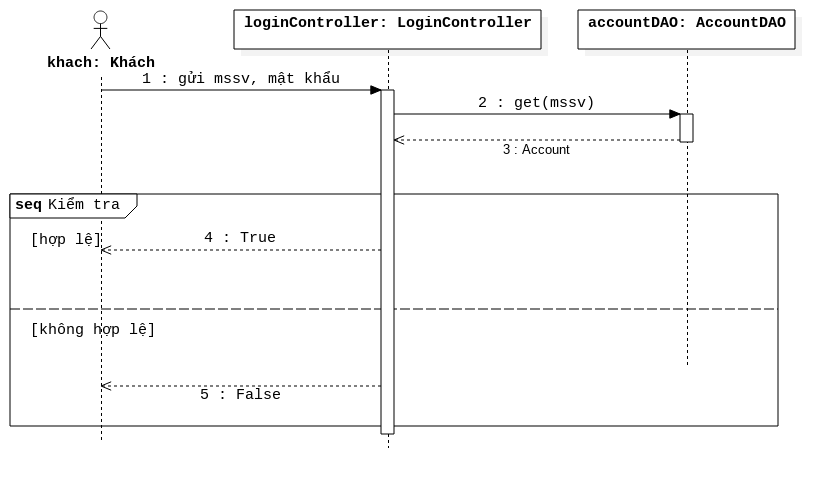
\includegraphics[width=15cm]{figures/dangnhapseq.png}
\caption{Trình tự đăng nhập}
\end{figure}

\begin{figure}[H]
\centering
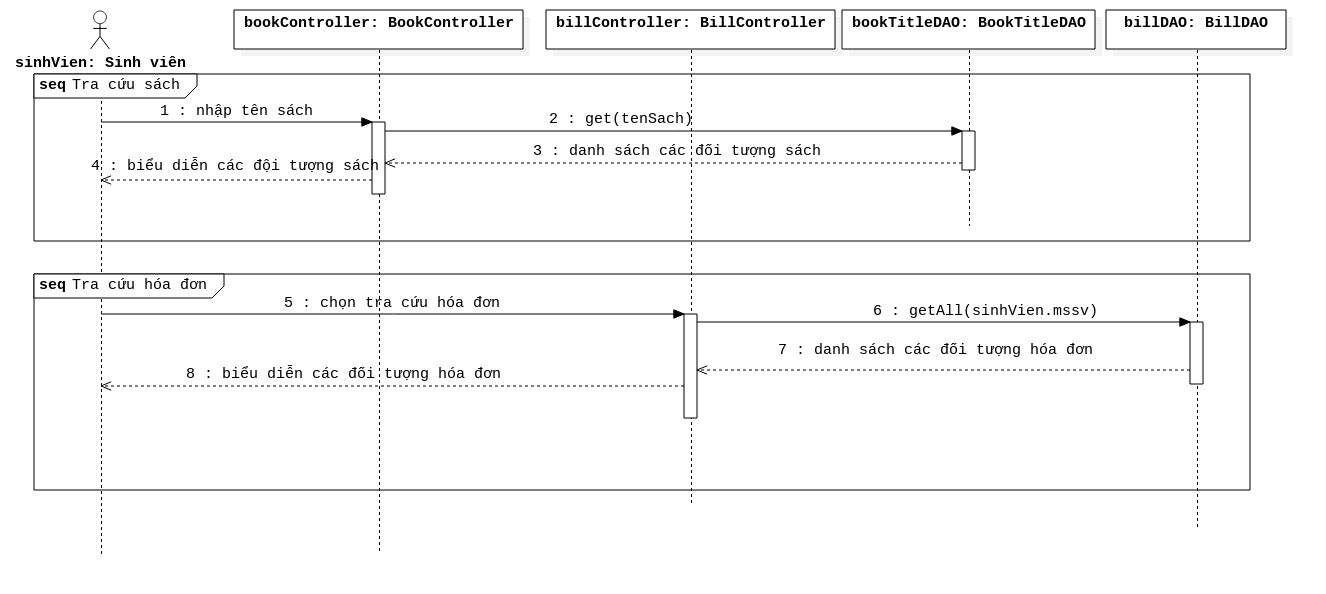
\includegraphics[width=\textwidth]{figures/tracuuseq.png}
\caption{Trình tự tra cứu}
\end{figure}

\begin{figure}[H]
\centering
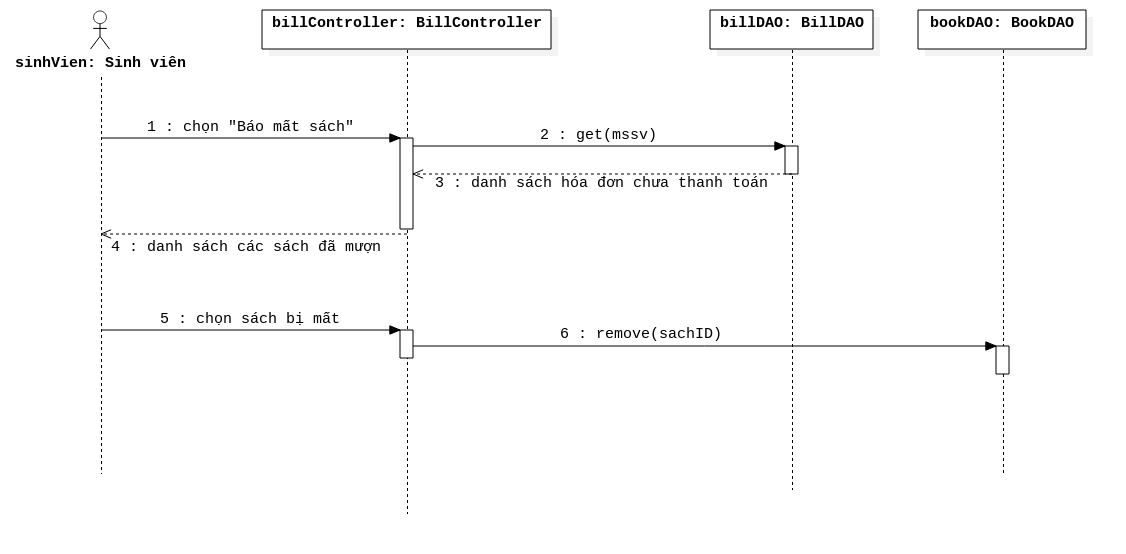
\includegraphics[width=\textwidth]{figures/baomatsachseq.png}
\caption{Trình tự báo mất sách}
\end{figure}

\begin{figure}[H]
\centering
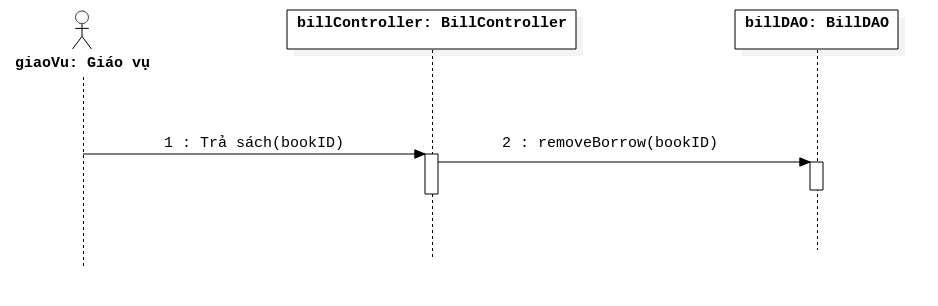
\includegraphics[width=\textwidth]{figures/nhantrasachseq.png}
\caption{Trình tự nhận trả sách}
\end{figure}

\begin{figure}[H]
\centering
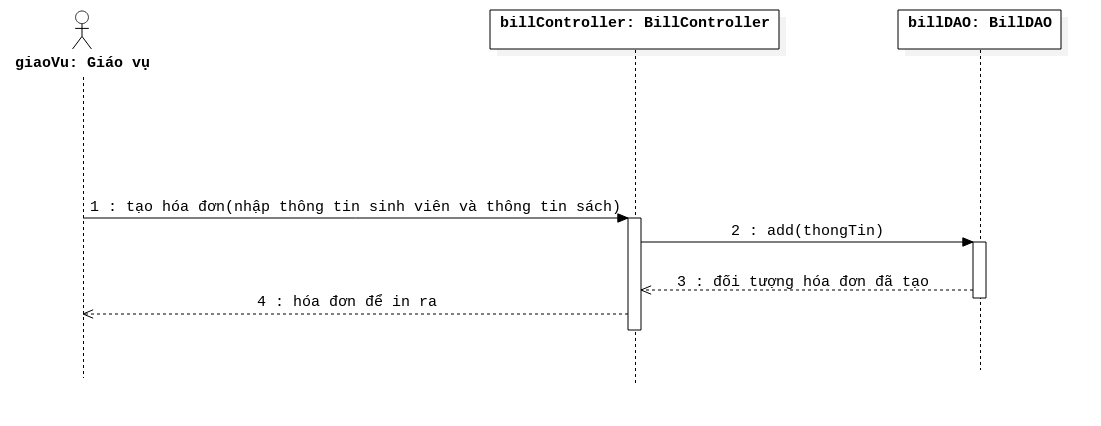
\includegraphics[width=\textwidth]{figures/taohoadonseq.png}
\caption{Trình tự tạo hóa đơn}
\end{figure}

\begin{figure}[H]
\centering
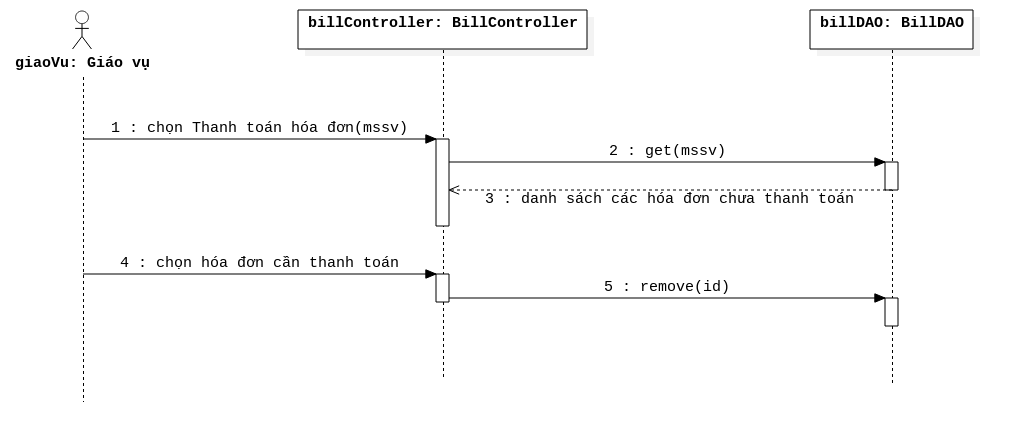
\includegraphics[width=\textwidth]{figures/thanhtoanseq.png}
\caption{Trình tự thanh toán hóa đơn}
\end{figure}

\begin{figure}[H]
\centering
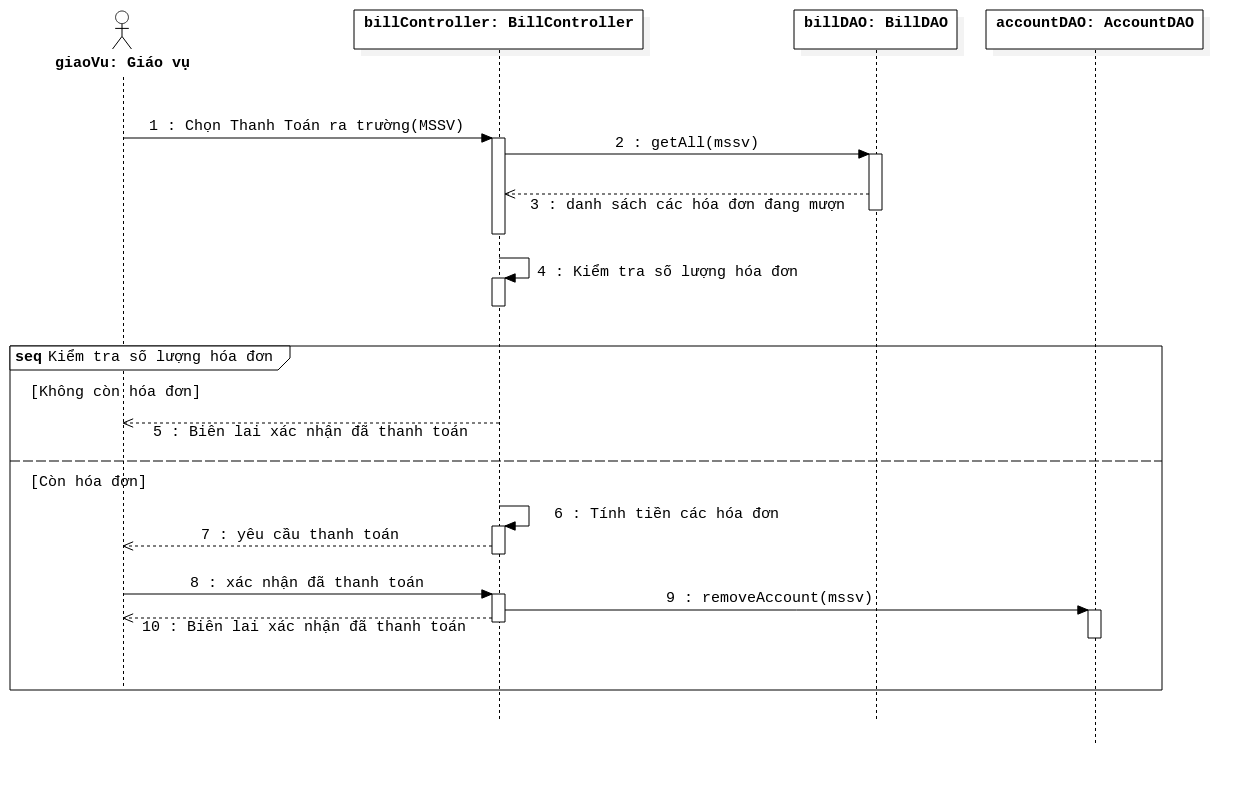
\includegraphics[width=\textwidth]{figures/thanhtoanratruongseq.png}
\caption{Trình tự thanh toán ra trường}
\end{figure}

\begin{figure}[H]
\centering
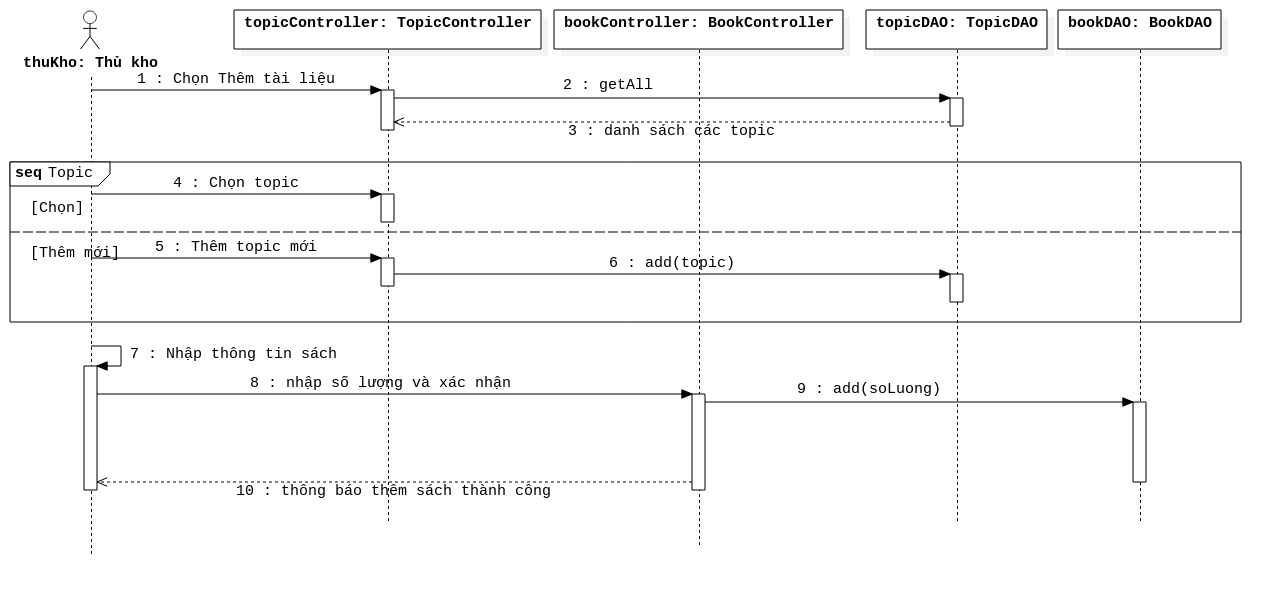
\includegraphics[width=\textwidth]{figures/themTlseq.png}
\caption{Trình tự thêm sách}
\end{figure}

\subsection{Biểu đồ communication}

\section{Mô hình thiết kế}
\subsection{Cơ sở dữ liệu}
Dựa trên phân tích nghiệp vụ ta thấy rằng, hệ thống cần quản lý các thông 
tin về các tài nguyên bao gồm: Thông tin sách, Thông tin tài khoản, 
Thông tin hóa đơn.
Tài khoản sẽ chứa thông tin về id tài khoản, mật khẩu và quyền mà 
tài khoản đang sở hữu.
Hóa đơn bao gồm các thông tin: số hiệu hóa đơn, ngày mượn, 
số tiền ký gửi và danh sách các sách được mượn.
Sách chứa thông tin về tên sách, chủ đề sách, 
giá sách và nguồn gốc của sách. 

Do có nhiều cuốn sách có cùng tên và với một topic sẽ có nhiều sách có tiêu đề khác nhau,
vì thế ở đây chúng ta sẽ sử dụng ba bảng để lưu thông tin về sách. 
\begin{itemize}
      \item Topic: chứa thông tin các chủ đề sách.
\item BookTitle: chứa thông tin về một tiêu đề sách.
\item Book: chứa thông tin để xác định một cuốn sách và trạng thái 
hiện tại của sách (được phép mượn hay không).

\end{itemize}


Một hóa đơn có thể chứa một hay nhiều cuốn sách và ngược lại, trong một khoảng 
thời gian nào đó thông tin của một sách sẽ chỉ được tìm thấy trong một hóa đơn duy nhất. 
Do vậy cần thêm một bảng để mô tả quan hệ giữa hóa đơn và sách.
 Bản thiết kế cơ sở dữ liệu thu được sẽ như sau:
\begin{figure}[H]
\centering
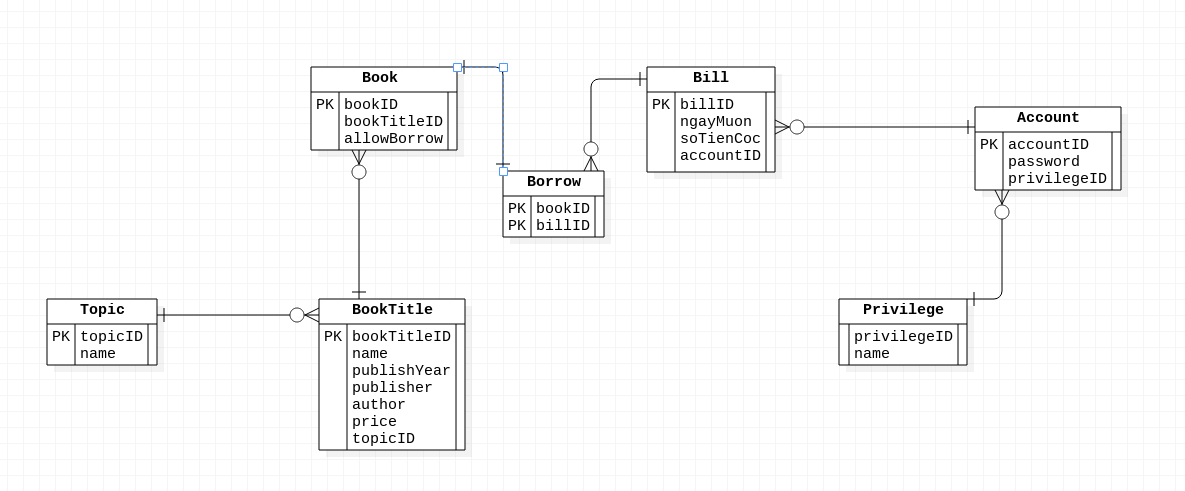
\includegraphics[width=\textwidth]{figures/db.png}
\caption{Thiết kế cơ sở dữ liệu trong hệ thống thư viện}
\end{figure}



\end{document}
